\section{Finding a conserved quantity for the SIRP model}
\label{app:P_exact}

Starting with the SIRP model,
\begin{equation}\label{eq:SIRP2}
    \begin{aligned}
        \dot{S} & =-\bar{\beta} P S                    \\
        \dot{I} & =\bar{\beta} P S-\gamma I            \\
        \dot{R} & =\gamma I                            \\
        \dot{P} & =\lambda I-\bar{\beta}P S -\mu P \ ,
    \end{aligned}
\end{equation}
from the $\dot{S}$ equation, $P$ can be written as follows,
\begin{equation}\label{eq:P_rel}
    P=-\frac{1}{\bar{\beta}}\frac{\dot{S}}{S} \ ,
\end{equation}
and summing up the equations for $\dot{S}$ and $\dot{I}$ the following
relation for $I$ is obtained
\begin{equation}\label{eq:I_rel}
    I=-(\dot{S}+\dot{I})/\gamma \ .
\end{equation}
Replacing \cref{eq:P_rel}, \cref{eq:I_rel} and the differential equation
for $\dot{S}$ in the $4$th differential equation in \cref{eq:SIRP2} one
obtains,
\begin{equation}
    \dot{P}=-{{\lambda}\over{\gamma}} (\dot{S}+\dot{I})+\dot{S}+
    {{\mu}\over{\bar{\beta}}}\ . {{\dot{S}}\over{S}}
\end{equation}
As $\dot{S}/S=d(\ln S)/dt$, all terms in the previous equation are exact
differentials with respect to time, and the equation can be integrated
yielding,

\begin{equation}
    P + \frac{\lambda}{\gamma}\parentesi{S+I}-S-\frac{\mu}{\bar{\beta}}\ln S=C
    \label{eq:conservedquantity_nacras_I}
\end{equation}
with the integration constant $C$,
that is a conserved quantity, i.e., it takes the same value at one time of
the dynamical evolution of the system.
$C$ is related to the initial conditions by,
\begin{equation}
    C = P(0)+\frac{\lambda}{\gamma}\parentesi{S(0)+I(0)} -
    \frac{\mu}{\bar{\beta}}\ln{S(0)} -
    S(0)=P(0)+\frac{\lambda}{\gamma}\parentesi{N-R(0)} -
    \frac{\mu}{\bar{\beta}}\ln{S(0)} - S(0)
    \label{eq:C_constant}
\end{equation}

It is possible to use \cref{eq:conservedquantity_nacras_I}-\cref{eq:C_constant}
to
express one of variables as a function of the others, for example
the parasite concentration $P$ as,
\begin{equation} \label{eq:PSI_exact}
    P(S, I)=P(0)-\frac{\lambda}{\gamma}\left(S+I-N+R(0)\right)+
    \frac{\mu}{\bar{\beta}}\ln{\frac{S}{S(0)}} + S - S(0)\ ,
\end{equation}
or equivalently as,
\begin{equation}\label{eq:psrexact}
    P(S,R)=P(0) + \frac{\lambda}{\gamma}\claudator{R-R(0)+
        \frac{\mu\gamma}{\bar{\beta}\lambda}\ln{\frac{S}{S(0)}}} + S - S(0)
\end{equation}

From \cref{eq:conservedquantity_nacras_I}, it is easy to show that the SIP
model
of Ref. \cite{article_SIP}, that differs from the SIRP model in that the
fourth equation is simplified to $\dot{P}=\lambda I-\mu P$, has as
exact conserved quantity,
\begin{equation}
    P + \frac{\lambda}{\gamma}\parentesi{S+I}-\frac{\mu}{\bar{\beta}}\ln
    S={\mathcal C}
    \label{eq:conservedquantitySIP}
\end{equation}
as the extra term in the SIRP model $-\bar{\beta}SP$ is equal to $\dot{S}$
from the first equation \cref{eq:SIRP2}.

The SIR model has a conserved quantity \cite{Murray_book}, that in the case
of
\cref{eq:SIRslow} takes the form,
\begin{equation}
    I+S-{{\gamma}\over{\beta'}} \ln S =C\ .
    \label{eq:SIRconservedquantity}
\end{equation}
Rewriting \cref{eq:conservedquantity_nacras_I} in the alternative form,
\begin{equation}
    {{\gamma}\over{\lambda}} P +\left(1-{{\gamma}\over{\lambda}}\right) S + I
    -{{\mu\gamma}\over{\lambda\bar{\beta}}} \ln S=C'
    \label{eq:conservedquantity2}
\end{equation}
it can be seen that if $\lambda>>\gamma$ \cref{eq:conservedquantity2} reduces
to
\cref{eq:SIRconservedquantity}, remembering that in \cref{eq:SIRslow}
$\beta'=\lambda\bar{\beta}/\mu$. The assumptions used to arrive to
\cref{eq:SIRconservedquantity} in \cref{sec:fastslow} where
$\mu>>(\gamma,\bar{\beta})$, and taking into account the expression for $R_0$
\cref{eq:R_0_SIRP}, that $\lambda\gtrsim\mu$ is most plausible to keep $R_0$
above the epidemic threshold ($R_0>1)$.

\section{Stability analysis of the fixed points of the SIRP model}
\label{app:linstabfp}

Here we will assume the initial fixed point of our SIRP model, with
$I(0)=P(0)=0$ right before the introduction of the infection, either through
$I$ or $P$.
We will assume that $R(0)=0$, so that $S(0)=N$.
To study the linear stability of the model we need to write the Jacobian, that
takes the form,
\begin{equation}
    J=
    \begin{pmatrix}
        -\bar{\beta} P & 0       & 0 & \bar{\beta} S       \\
        \bar{\beta} P  & -\gamma & 0 & \bar{\beta} S       \\
        0              & \gamma  & 0 & 0                   \\
        -\bar{\beta} P & \lambda & 0 & (\bar{\beta} S-\mu)
    \end{pmatrix}
\end{equation}
and obtain the eigenvalues for both fixed points, where we have already used
the standard incidence, $\bar{\beta}=\beta/N$, from the evidence of the
validation with experiments.
For the pre-epidemic fixed point, the Jacobian becomes,
\begin{equation}
    \begin{pmatrix}
        0 & 0       & 0 & \bar{\beta} S(0)       \\
        0 & -\gamma & 0 & \bar{\beta} S(0)       \\
        0 & \gamma  & 0 & 0                      \\
        0 & \lambda & 0 & (\bar{\beta} S(0)-\mu)
    \end{pmatrix}
    \label{eq:Jacobian}
\end{equation}
Matrix \cref{eq:Jacobian} has two null $(0$) eigenvalues and a pair of
eigenvalues given by,
\begin{equation}
    \Lambda_{1,2}=-{1\over 2}\left(\gamma+\mu+{{\bar{\beta}
                S(0)}}\pm\sqrt{\gamma^2+\mu^2+\left({{\bar{\beta}
                    S(0)}}\right)^2
        +{{2\mu\bar{\beta} S(0)}}-2\gamma\mu
        -{{2\gamma\bar{\beta} S(0)}}+{{4\lambda\bar{\beta} S(0)}}}
    \right)
\end{equation}
from which one can determine that the fixed point is unstable whenever
\begin{equation}
    \lambda\bar{\beta} S(0)>\gamma(\mu+\bar{\beta} S(0))
    \label{eq:eigenvineq}
\end{equation}
and stable if the inequality is reversed.
It can be easily shown that \cref{eq:eigenvineq} is equivalent to $R_0>1$, with
$R_0$ given by \cref{eq:R_0_SIRP}.

The final point of the epidemic,  $S(\infty)$, can be found by solving the
transcendental equation,
\begin{equation}
    \left({{\lambda}\over{\gamma}}-1\right)S(\infty)
    -\frac{\mu}{\bar{\beta}}\ln (S(\infty))=C
    \label{eq:sinftytreqn}
\end{equation}
where $C$ is determined from the initial conditions (\cref{eq:C_constant})
and $I(\infty)=P(\infty)=0$.
(\cref{eq:sinftytreqn}) has two roots, where $S({\infty})$ represents the
smallest one.

\section{Calculation of $R_0$ using the Next Generation Matrix
  method}\label{app:NGM}

The so called Next Generation Method (NGM) is a method to obtain $R_0$, the
basic epidemiological quantity that measures the number of secondary cases
produced by a typical infected individual during its entire period of
infectiousness in a completely susceptible population. It was discussed in
\cref{app:linstabfp} that $R_0$ is related to the largest non-zero eigenvalue,
say $\Lambda$, of the fixed point corresponding to the infection-free
equilibrium. An outbreak occurs when $\Lambda>0$ (or equivalently when $R_0>1$)
and the NGM is an ingenious method to obtain directly $R_0$ in a reduced linear
system.
In more concrete terms, within the NGM method $R_0$ is the dominant eigenvalue
of a suitably defined linear operator (a linear matrix in a suitable basis).
This operator is obtained from a decomposition of the Jacobian, $J$ of
the infected/infecting compartments (i.e. excluding susceptible and removed
compartments) in the form $J=T+\Sigma$, where $T$ is
the
\textit{transmission part}, that describes the production of new infections,
and $\Sigma$  the \textit{transition part}, that describes changes of
state (including death). Then, it can be proved \cite{Diekmann2010} that the
\textit{basic reproduction number} $R_0$ is given by the spectral radius (i.e.
the largest eigenvalue) of the (next generation) matrix $K=- T
    \Sigma^{-1}$.

In the case of the SIRP model the decomposition is applied to the $2\times 2$
Jacobian corresponding to the dynamical evolution of the $(I,P)$
\textit{infectious} compartments, being the decomposition,
\begin{equation*}
    J=\parentesi{\begin{array}{cc}
            -\gamma & \bar{\beta} S_0        \\
            \lambda & -(\bar{\beta} S_0+\mu)\end{array}}\qquad
    T=\parentesi{\begin{array}{cc}
            0 & \bar{\beta} S_0 \\
            0 & 0
        \end{array}} \qquad \Sigma=\parentesi{\begin{array}{cc}
            -\gamma & 0                        \\
            \lambda & -(\bar{\beta} S_0 + \mu)
        \end{array}}
\end{equation*}
where the $\bar{\beta} PS$ term in $\dot{I}$ is the only one that contributes
to the transmission matrix, as it is the only process involving infection,
while all the other terms in the dynamical equations of $\dot{I}$ and $\dot{P}$
imply transitions (to another compartment, like $I\rightarrow R$ or birth and
death of $P$).

Then, the next generation matrix is given by,
\begin{equation*}
    K=- T\Sigma^{-1}=\parentesi{\begin{array}{cc}
            \displaystyle \frac{\lambda\beta S_0}{\gamma(\beta S_0 + \mu)} &
            \displaystyle \frac{\beta S_0}{\beta S_0 + \mu}
            \\
            0                                                              & 0
        \end{array}} \Longrightarrow R_0=\frac{\lambda \beta
        S_0}{\gamma\parentesi{\beta S_0+\mu}} \ ,
\end{equation*}
This result coincides with the expectation that $R_0$ should correspond to the
number of  hosts infected in a single generation by the appearance of an
infected host in a completely susceptible population. This can be obtained from
the number of parasites produced by an infected host, $\lambda$, times the time
in which the infected host is alive producing parasites, $1/\gamma$, multiplied
by the number of infected hosts produced per parasite, $\beta S_0$, times the
time the parasite is alive available to infect, $1/(\mu+\beta S_0)$, taking
into account that parasites are inactivated at a rate $\mu$ and also die when
infecting at a rate $\beta S_0$, where this result assumes that the susceptible
population does not change from its initial value $S_0$.

\section{Sensitivity Analysis} \label{app:sensanal}

One particular way to analyse the local sensitivity (LSA) of a given model
function, $F(\vec{p})$, for each of the parameters that conform it, $p_i$, is
through the normalised sensitivity indexes \cite{sensitivity_analysis},
\begin{equation}\label{eq:sensitivity_analysis}
    \Omega_{p_i}^{F}=\dpart{F}{p_i}\frac{p_i}{F}\Big|\limitss{p_i=p^0}{} \
    .
\end{equation}
where the partial derivatives in \cref{eq:sensitivity_analysis} are
determined analytically in our case.

GSA works by studying the influence of a large domain of parameter space in
the final state of the epidemic and in the epidemic peak.
In our case this will be achieved by means of a variance based analysis,
known as Sobol method \cite{SOBOL2001271}. This particular method provides
information no only on how a particular parameter alone influences the model
outputs (as happens with LSA), but also on the influence of its interactions
with other parameters. This information is organised in what are known as Sobol
indices, that have been
implemented within the Julia high-level programming language \cite{julia}
using the DifferentialEquations.jl package \cite{DifferentialEquations.jl},
and in particular through its subpackage DiffEqSensitivity.jl. This
implementation allows the user to sample the parameter space using
QuasiMonteCarlo methods and thus obtain confidence intervals (CI) for the
sensitivity indices, which are directly related to the committed statistical
error.

The total order indices are a measure of the total variance of the output
quantity caused by variations of the input parameter and its interactions.
First order (or ``main effect'') indices are a measure of the contribution to
the output variance given by the variation of the parameter alone, but averaged
over variations in other input parameters. Second order indices take into
account first order interactions between parameters. Further indices can be
obtained, describing the influence of higher-order interactions between
parameters, but these are not going to be considered.
More detailed information about sensitivity analysis can be found in
\cite{Sensitivity_analysis_book}.

\section{General rate change with temperature} \label{app:rate_change}

In \cite{Gillooly2248} the metabolic rate of a wide variety of organisms
was studied, showing that the change in the metabolic rate with temperature was
similar among them. In particular, the natural logarithm of the metabolic rate
linearly depends on the inverse of absolute temperature,
\begin{equation}
    \log(R(T))=a\cdot\parentesi{\frac{100}{T}}+b
\end{equation}
and for all the analysed organisms they found that $a$ lies between $-5$
and $-10$ and $b$ between $14$ and $30$. From their analysis, we can compute
the change in the rate for a given increase of temperature,
\begin{equation}\label{eq:rate_change}
    \frac{R(T+\Delta T)}{R(T)}=\exp(a\cdot\parentesi{\frac{100}{T + \Delta
            T}}+b) / \exp(a\cdot\parentesi{\frac{100}{T}}+b) = \exp(a \cdot
    \frac{-1000}{T+\Delta T}\cdot \frac{\Delta T}{T}) \ .
\end{equation}
Substituting $T=287 K$ and $\Delta T=3 K$, that correspond to our available
data (cf. \cref{sec:validation}) in \cref{eq:rate_change}, using both the upper
and lower limit of $a$, we obtain that the expected increase in the effective
transmission rate is between $1.2$ to $1.4$. This is far from the $19$-fold
increase that we obtained with the mass action hypothesis in
\cref{sec:validation}
while it is in good agreement with either the $1.92$ ratio we obtained	for
$\bar{\beta}$ with the reduction of \cref{sec:exactredapp} or the $1.43$ ratio
obtained with the fast-slow approximation of \cref{sec:fastslow}, both obtained
using the standard incidence choice.

\cref{fig:rate_changes}(a) shows the change in the rate with an increase of
$\SI{3}{\degree C}$ for different base temperatures and for all the organisms
analysed in \cite{Gillooly2248}, and using their fit. Note that for all
temperatures between $\SI{0}{\degree C}$  and $\SI{30}{\degree C}$ the rate
change lies between $1.2$ and $1.45$. \cref{fig:rate_changes}(b) shows the
change in the rate for different temperature increases, with a base temperature
of $T=\SI{287}{K}$. Note that in order to obtain a $19$-fold increase the
temperature change should be at least of $\SI{30}{\degree C}$\footnote{A
    temperature change of $\SI{30}{\degree C}$ could fall outside the range in
    which the study of \cite{Gillooly2248} is valid. We just stress that a
    $19$-fold rate change is unlikely for the case of a $\SI{3}{\degree C}$
    that
    correspond to the $2$ data sets that we compare in this section.}.
The temperature dependence of metabolic rates has been reported in the
context of epidemic parameters \cite{COELHO2006,Shapiro2017}

The behavior of the metabolic rates re-analysed here has been also found
experimentally in epidemic contexts such as \cite{COELHO2006, Shapiro2017},
i.e. the increase of the rates with temperature fulfill the ranges shown here.

\begin{figure}[H]
    \centering
    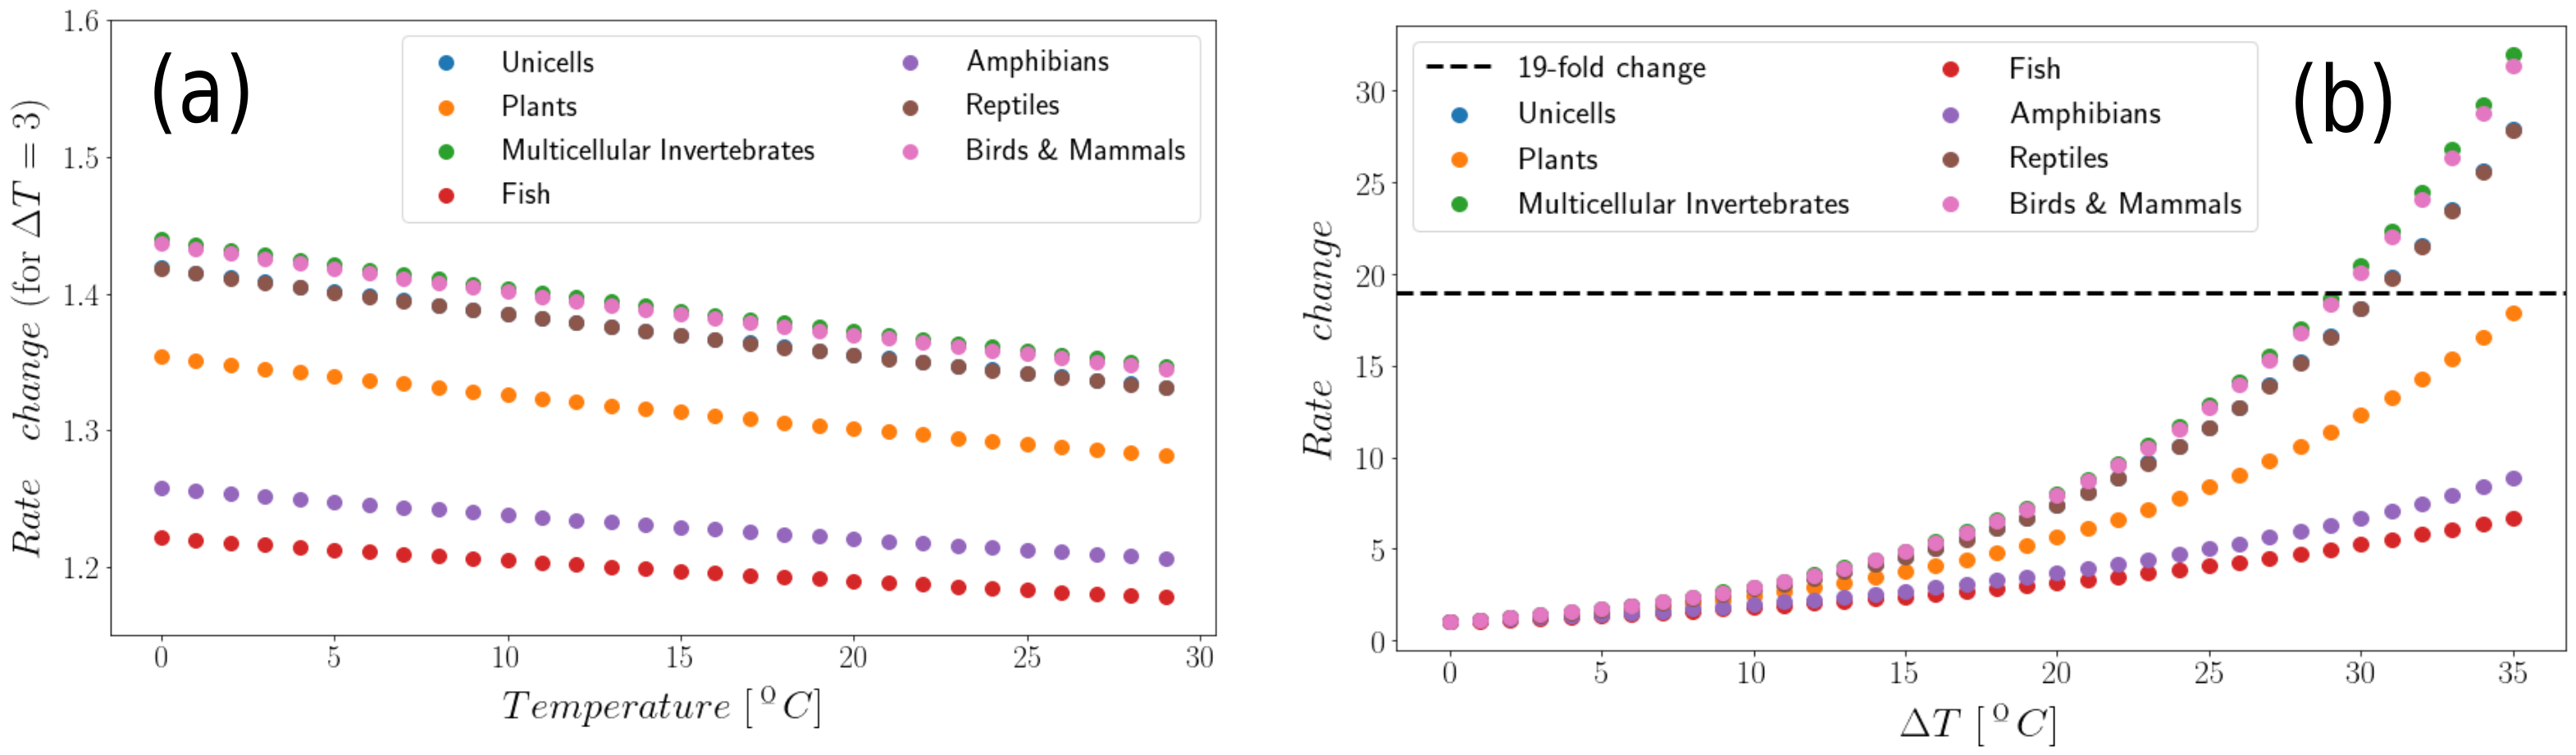
\includegraphics[width=1\textwidth]{Figures/arrhenius.png}
    \caption{Graphical representation of change in the rate (in ordinates)
        for different reference temperatures (in abscissae) for: (a) a
        temperature
        increase of $\SI{3}{\degree C}$; (b)  a temperature increase of
        $\SI{14}{\degree C}$. The black dotted line in (b) corresponds to a
        $19$-fold
        increase in the rate.
    }
    \label{fig:rate_changes}
\end{figure}

\section{Derivation of the non-spatial equation for $R_{\infty}$}
\label{app:Rinf}

The model described by the ODE system in \cref{eq:SIRP_MF} has a conserved
quantity $\mathcal{C}$ given by \cite{GimenezRomero2021}.
\begin{equation}\label{eq:conservedquantity}
    \mathcal{C}=P +
    \frac{\lambda}{\gamma}\parentesi{S+I}-S-\frac{\mu}{\bar{\beta}}\ln S
\end{equation}

At $t=\infty$ the system reaches an absorbing state completely determined
by $S(\infty)$, as $P(\infty)=I(\infty)=0$ and $N=S(\infty)+R(\infty)$. Thus,
from \cref{eq:conservedquantity} we have
\begin{equation}\label{eq:transcendental}
    S(\infty)\parentesi{\frac{\lambda}{\gamma}-1}-
    \frac{\mu}{\beta}\ln(S(\infty))=\mathcal{C}_0
\end{equation}

The transcendental equation \cref{eq:transcendental} can be solved by means
of the Lambert's W function,
\begin{equation}
    S(\infty)=-\frac{\mu\gamma}{\beta\parentesi{\lambda-\gamma}}
    W_0\parentesi{-\frac{\beta\parentesi{\lambda-\gamma}}{\mu\gamma}
        \exp(-\beta\mathcal{C}_0/\mu)}
\end{equation}
which can be simplified to
\begin{equation}\label{eq: S_inf}
    S(\infty)=-\frac{S(0)}{\xi}W_0\parentesi{-\xi\exp(-\frac{\beta}{\mu}C)}
    \ ,
\end{equation}
with $\xi=S(0)\frac{\beta\parentesi{\lambda-\gamma}}{\mu\gamma}$ and
$C=P(0)+\frac{\lambda}{\gamma}\parentesi{S(0)+I(0)}-S(0)$.\\

Finally, the absorbing state fulfils the condition $N=S(\infty)+R(\infty)$
so that the final number of dead individuals can be expressed as
\begin{equation}
    R(\infty)=N+\frac{S(0)}{\xi}W_0\parentesi{-\xi\exp(-\frac{\beta}{\mu}C)} \
    .
\end{equation}